\subsection*{Problema 23}

\textbf{Enunciado:} Calcular la integral:
\begin{align*}
  \int \dfrac{dx}{\sqrt{x^2 + 2x \cos\alpha + 1}}
\end{align*}

\textbf{Solución:} \newline
Completamos el cuadrado en el trinomio del denominador. 
Tomamos los términos con $x$:
\begin{align*}
  x^2 + 2x \cos\alpha
\end{align*}

Sumamos y restamos el cuadrado de la mitad del coeficiente de $x$, es decir, $(\cos\alpha)^2$:
\begin{align*}
  x^2 + 2x \cos\alpha + \cos^2\alpha - \cos^2\alpha + 1
\end{align*}

Agrupamos los tres primeros términos como un trinomio cuadrado perfecto y simplificamos los restantes usando la identidad fundamental:
\begin{align*}
  (x + \cos\alpha)^2 + (1 - \cos^2\alpha) \\
  = (x + \cos\alpha)^2 + \sin^2\alpha
\end{align*}

Sustituimos este resultado en el denominador de la integral original:
\begin{align*}
  \int \dfrac{dx}{\sqrt{(x + \cos\alpha)^2 + \sin^2\alpha}}
\end{align*}

Aplicamos la fórmula de integración estándar para integrales de la forma $\int \dfrac{du}{\sqrt{u^2 + a^2}}$, donde $u = x + \cos\alpha$, $du = dx$ y $a = \sin\alpha$:
\begin{align*}
  \int \dfrac{du}{\sqrt{u^2 + a^2}} = \ln\left|u + \sqrt{u^2 + a^2}\right| + C
\end{align*}

Sustituyendo de regreso las variables originales:
\begin{align*}
  \ln\Big|(x + \cos\alpha) + \\
  \sqrt{(x + \cos\alpha)^2 + \sin^2\alpha}\Big| + C
\end{align*}

Simplificando la expresión dentro del radical:
\begin{align*}
  \ln\Big|x + \cos\alpha + \\
  \sqrt{x^2 + 2x \cos\alpha + 1}\Big| + C
\end{align*}

\textbf{Resultado Final:}
\begin{align*}
  \int \dfrac{dx}{\sqrt{x^2 + 2x \cos\alpha + 1}} = \\
  \ln\Big|x + \cos\alpha + \sqrt{x^2 + 2x \cos\alpha + 1}\Big| + C
\end{align*}

\begin{figure}[H]
	\centering
	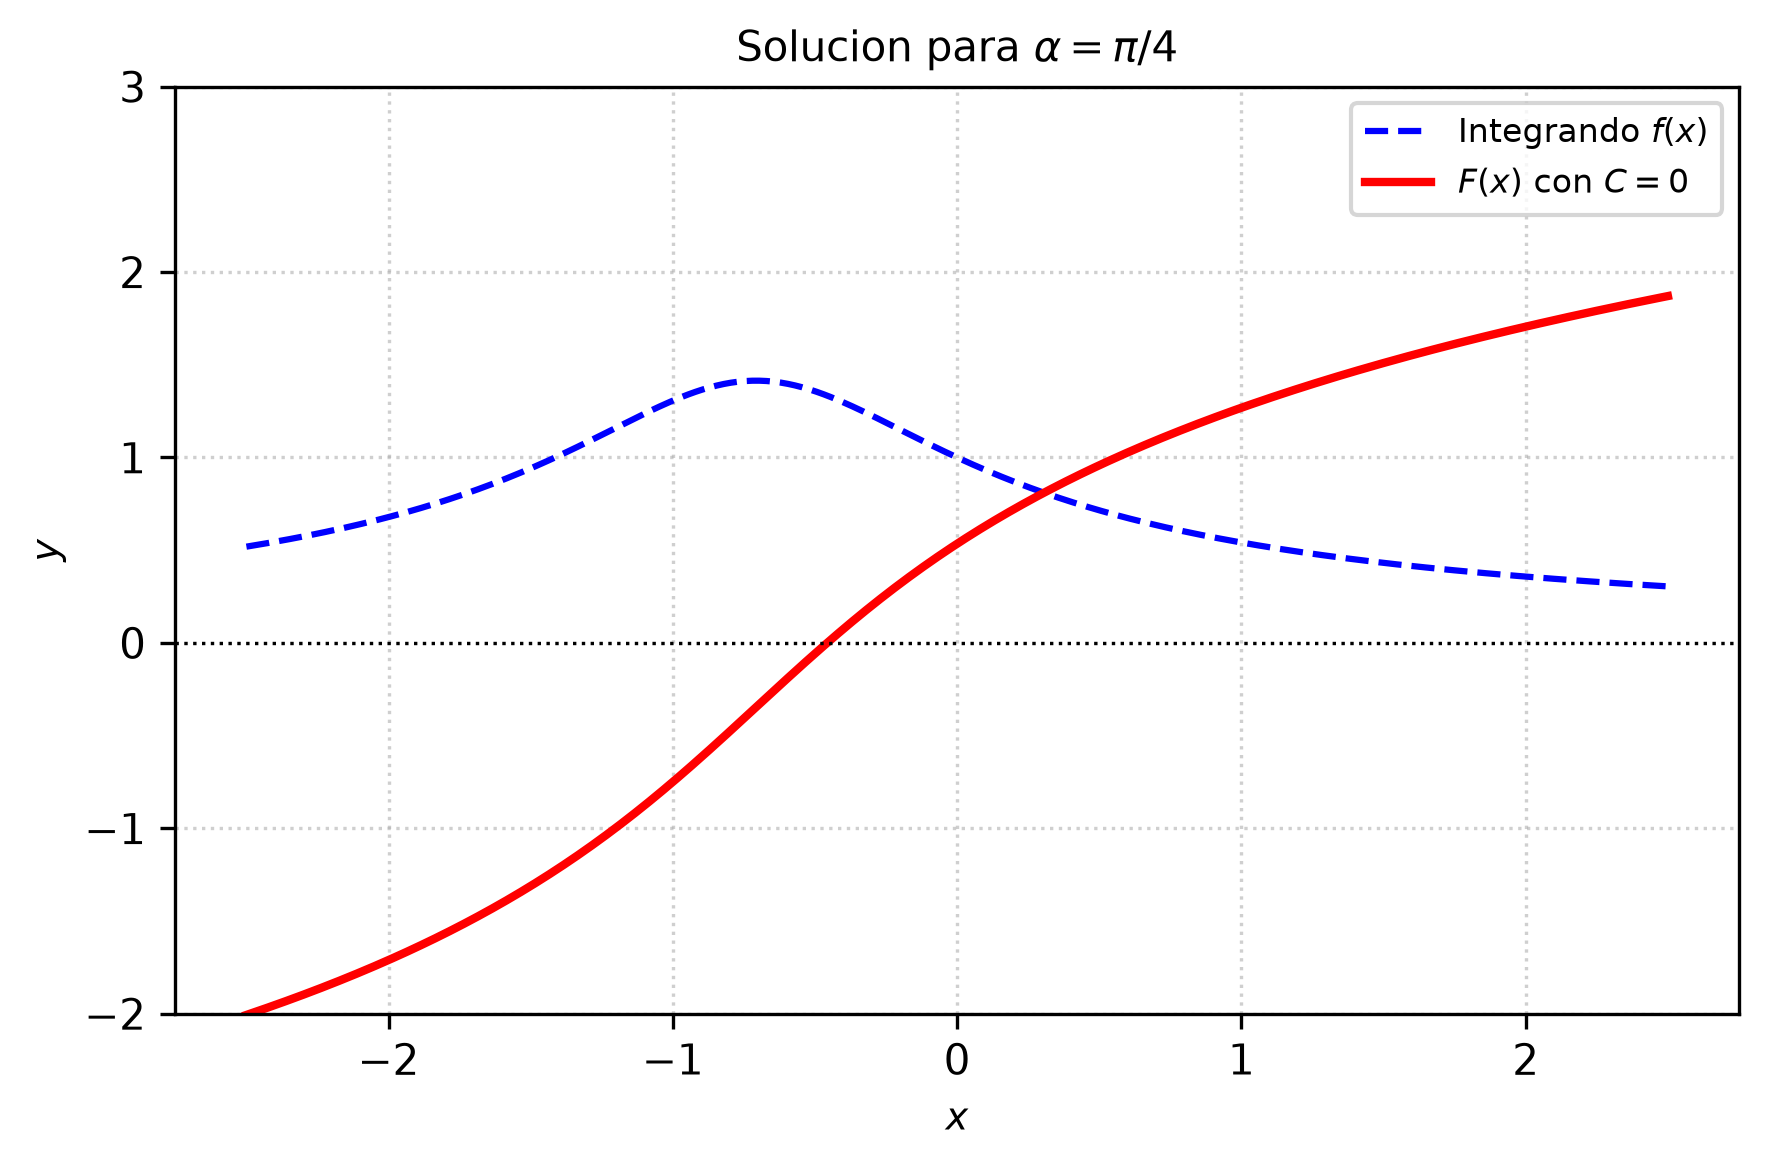
\includegraphics[width=\columnwidth]{semana_05/graficas/SEM05_P23_grafica.png}
	\caption{Representación gráfica de $f(x)$ y su antiderivada $F(x)$ evaluada para la constante de integración $C = 0$ (Problema 23).}
	\label{fig:problema23}
\end{figure}
